\documentclass[11pt]{article}

\usepackage{amsmath}
\usepackage{amssymb}
\usepackage{array}
\usepackage{geometry}
\usepackage{enumitem}
\usepackage{float}
\usepackage{cancel}
\usepackage{graphicx}
\usepackage[labelformat=empty]{caption}

\geometry{
	a4paper,
 	left=20mm,
 	top=20mm,
}

\setlength{\parindent}{0pt}

\begin{document}

\section{Trigonometrie}

\begin{equation*}
\begin{split}
	\sin(0) = 0,\ \sin(\frac{\pi}{4}) = \frac{\sqrt{2}}{2},\ \sin(\frac{\pi}{2}) & = 1,\ \sin(\pi) = 0,\ \sin(\frac{3\pi}{4}) = \frac{\sqrt{2}}{2}\\
	\cos(0) = 1,\ \cos(\frac{\pi}{4}) = \frac{\sqrt{2}}{2},\ \cos(\frac{\pi}{2}) & = 0,\ \cos(\pi) = -1,\ \cos(\frac{3\pi}{4}) = -\frac{\sqrt{2}}{2}\\
\end{split}
\end{equation*}

\begin{equation*}
\begin{split}
	\tan(x) & = \frac{\sin(x)}{\cos(x)} \\
	\sin(2x) & = 2\sin(x)\cos(x) \\
	\sin(\alpha + \beta) & = \sin(\alpha)\cos(\beta) + \cos(\alpha)\sin(\beta) \\
	\cos(\alpha + \beta) & = \cos(\alpha)\cos(\beta) + \sin(\alpha)\sin(\beta) \\
	\cos^2(x) & = \frac{1 + \cos(2x)}{2} \\
	\sin^2(x) + \cos^2(x) & = 1
\end{split}
\end{equation*}

\section{Mengen}

\subsection{Definitionen}

\begin{description}[labelindent=16pt,style=multiline,leftmargin=6cm, noitemsep]
	\item[Obere/Untere Schranke:] $\exists b \in \mathbb{R}\ \forall a\in A:\ a \leq b$, $\exists c \in \mathbb{R}\ \forall a\in A:\ a \geq c$
	\item[Supremum:] kleinste obere Schranke $\sup A$
	\item[Infimum:] gr{\"o}sste untere Schranke $\inf A$
	\item[Maximum/Minimum:] $\sup A \in A$, $\inf A \in A$
\end{description}

\subsection{Identitäten}

\begin{equation*}
\begin{split}
	A + B & := \{a + b | a \in A, b \in B\} \\
	\sup(A+B) = \sup A + \sup B,\ & \inf(A+B) = \inf A + \inf B \\
	\sup(A \cup B) = \max\{\sup A, \sup B\},\ & \inf(A \cup B) = \min\{\inf A, \inf B\}
\end{split}
\end{equation*}

\section{Komplexe Zahlen}

\subsection{Polarform}

\begin{minipage}[c]{0.5\textwidth}
\centering
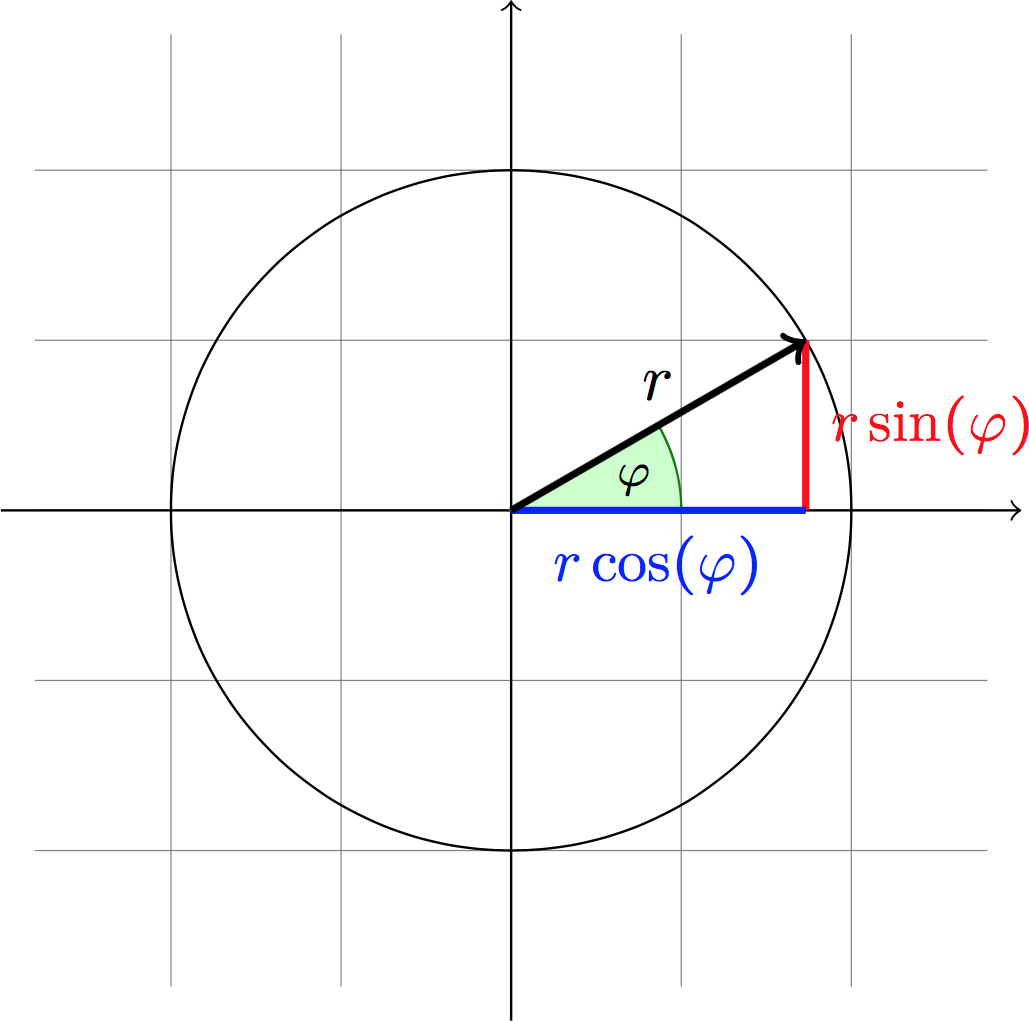
\includegraphics[width=\linewidth,keepaspectratio=true]{images/polarform}
\end{minipage}
%
\begin{minipage}[c]{0.5\textwidth}
\begin{equation*}
\begin{split}
	z & = x + iy = r(\cos(\varphi) + i\sin(\varphi)) = re^{i\varphi} \\
	r & = |z| = \sqrt{x^2 + y^2} \\
	\varphi & = \arctan(\frac{y}{x}) =  \\
	x & = r\cos(\varphi) \\
	y & = r\sin(\varphi) \\
	zw & = (re^{i\varphi})\cdot(se^{i\psi}) = rse^{i(\varphi + \psi)} \\
	\sqrt[q]{z} & = \sqrt[q]{s}e^{i\phi}\text{, wobei }\phi = \frac{\varphi}{q} \mod \frac{2\pi}{q} \\
	e^{i(\frac{\pi}{2} + 2\pi k)} & = i,\ e^{i\pi} = 1, \ e^{-i\pi} = -1
\end{split}
\end{equation*}
\end{minipage}

\subsection{Identit{\"a}ten}

\begin{equation*}
\begin{split}
	\overline{z} & = x - iy\\
	z^{-1} & = \frac{\overline{z}}{|z|^2} \\
	(a,b) \cdot (c, d) & = (ac-bd, ad+bc) \\
	i & = \sqrt{-1}\\
	i^2 & = -1 \\
	|z|^2 & = z\overline{z} \\
	|zw|^2 & = (zw) \cdot \overline{(zw)} = |z|^2|w|^2
\end{split}
\end{equation*}

\section{Grenzwert}

\subsection{Dominanz}

\begin{equation*}
\begin{split}
	\text{F{\"u}r}\ x \to +\infty:\quad & ... < \log(\log(x)) < \log(x) < x^\alpha < \alpha^x < x! < x^x \\
	\text{F{\"u}r}\ x \to 0:\quad & ... < \log(\log(x)) < \log(x) < (\frac{1}{x})^\alpha \\
\end{split}
\end{equation*}

\subsection{Tipps}

\begin{equation*}
\begin{split}
	\lim_{x \to a} \frac{\sin \odot}{\odot} & = 1\ \text{mit}\ \odot \xrightarrow{\: x \to a \: } 0 \\ 
	\lim_{x \to a} (1 + \frac{1}{\odot})^\odot & = e\ \text{mit}\ \odot \xrightarrow{\: x \to a \: } \infty \\ 
	\lim_{x \to a} (1 + \odot)^\frac{1}{\odot} & = e\ \text{mit}\ \odot \xrightarrow{\: x \to a \: } 0 \\ 
\end{split}
\end{equation*}

\subsection{Wurzeltrick}

\begin{equation*}
	\lim_{x\to\infty} \sqrt{\alpha}+\beta = \lim_{x\to\infty}(\sqrt{\alpha}+\beta)\frac{\sqrt{\alpha}-\beta}{\sqrt{\alpha}-\beta}
\end{equation*}

\subsection{$e^{\log(x)}$-Trick}

\paragraph{Anforderung:}Term der Form $f(x)^{g(x)}$ mit Grenzwert "$0^0$", "$\infty^0$" oder "$1^\infty$" f{\"u}r $x \to 0$

\begin{equation*}
	\textbf{Grundsatz:}\quad\lim_{x\to a}f(x)^{g(x)} = \lim_{x\to a}e^{g(x) \cdot \log(f(x))}
\end{equation*}

\subsection{Satz von Bernoulli-de l'H{\^o}pital}

\paragraph{Anforderung:}Term der Form $\frac{f(x)}{g(x)}$ mit Grenzwert entweder "$\frac{0}{0}$" oder "$\frac{\infty}{\infty}$" mit $g'(x) \neq 0$. \\
Falls die Grenzwerte $0 \neq \infty$ verschieden sind, kann man umformen: $\frac{f(x)}{\frac{1}{g(x)}}$.

\begin{equation*}
	\textbf{Grundsatz:}\quad\lim_{x\to a}\frac{f(x)}{g(x)} = \lim_{x\to a}\frac{f'(x)}{g(x)}
\end{equation*}

Zwei Polizisten zu benutzen mit sin, cos, tan oder $-1^n$... sonst induktion:$a_{n+1}\geq a_{n} \Rightarrow a_{n+2} \geq a_{n+1}$ oder direct. Mit eine recursive folge, um Grenzwert zu finden, setzen $a_n$ mit a und a finden. Oder direct mit $a_{n+1} - a_n \geq 0$.

\section{Reihen}

\subsection{Konvergenzkriterien}

\begin{table}[H]
\centering
\begin{tabular}{|p{5cm}|p{4cm}|p{5cm}|}
\hline
                                             & \textbf{Eignung}    & \textbf{Bemerkung}                        \\ \hline
\textbf{Limes des allgemeinen Glieds}        &                     & zeigt nur Divergenz                       \\ \hline
\textbf{Majoranten- und Minorantenkriterium} &                     & ersten Glieder spielen keine Rolle        \\ \hline
\textbf{Quotientenkriterium}                 & $a_n$ mit Faktoren wie $n!$, $a^n$, oder Polynome & gleiche Folgerung wie Wurzelkriterium     \\ \hline
\textbf{Wurzelkriterium}                     & $a_n = (b_n)^n$     & gleiche Folgerung wie Quotientenkriterium \\ \hline
\textbf{Leibnitz-Kriterium}                  & alternierende Reihe &                                           \\ \hline
\textbf{Absolute Konvergenz}                 & $\sin$, $\cos$	   &                                           \\ \hline
\end{tabular}
\end{table}
\subsubsection*{Limes des allgemeinen Glieds}

\paragraph{Bemerkung:} Mit dieser Methode lässt sich nur die Divergenz beweisen, nicht jedoch die Konvergenz.

\begin{enumerate}
	\item $\sum_n a_n$ gegeben
	\item Grenzwert $\lim_{n\mapsto\infty} a_n$ berechnen
	\begin{itemize}
		\item falls Grenzwert $\neq 0 \Rightarrow$ \textbf{divergent} 
		\item falls Grenzwert $= 0 \Rightarrow$ keine Aussage 
	\end{itemize}
\end{enumerate}

\subsubsection*{Majoranten- und Minorantenkriterium}

Es seien $a_n$, $b_n > 0$ mit $a_n \geq b_n\ \forall n$ ab einem gewissen $n_0$. Dann gilt: 
\begin{equation*}
\begin{split}
	\sum_n a_n \text{ konvergent} & \Rightarrow \sum_n b_n \textbf{ konvergent}\quad \text{(Majorantenkriterium)} \\
	\sum_n b_n \text{ divergent} & \Rightarrow \sum_n a_n \textbf{ divergent}\quad \text{(Minorantenkriterium)} \\
\end{split}
\end{equation*}

\subsubsection*{Vergleichskriterium}

\begin{enumerate}
	\item $\sum_n a_n$ und $\sum_n b_n$ gegeben mit $a_n,b_n > 0$
	\item Grenzwert $\lim_{n\mapsto\infty} \frac{a_n}{b_n}$ berechnen
	\begin{itemize}
		\item falls Grenzwert $= 0$:
		\begin{itemize}
			\item $\sum_n a_n$ divergent $\Rightarrow \sum_n b_n$ \textbf{divergent}
			\item $\sum_n b_n$ konvergent $\Rightarrow \sum_n a_n$ \textbf{konvergent}
		\end{itemize} 
		\item falls Grenzwert $= \infty$:
		\begin{itemize}
			\item $\sum_n a_n$ konvergent $\Rightarrow \sum_n b_n$ \textbf{konvergent}
			\item $\sum_n b_n$ divergent $\Rightarrow \sum_n a_n$ \textbf{divergent}
		\end{itemize} 
	\end{itemize}
\end{enumerate}

\subsubsection*{Quotientenkriterium}

\begin{enumerate}
	\item $\sum_n a_n$ mit $a_n \neq 0$ gegeben
	\item Grenzwert $\lim_{n\mapsto\infty}|\frac{a_{n+1}}{a_n}|$ berechnen
	\begin{itemize}
		\item falls Grenzwert $> 1 \Rightarrow$ \textbf{divergent}
		\item falls Grenzwert $< 1 \Rightarrow$ \textbf{konvergent}
		\item falls Grenzwert $= 1 \Rightarrow$ keine Aussage
	\end{itemize}
\end{enumerate}

\subsubsection*{Wurzelkriterium}

\begin{enumerate}
	\item $\sum_n a_n$ mit $a_n \neq 0$ gegeben
	\item Grenzwert $\lim_{n\mapsto\infty}\sqrt[n]{|a_n|}$ berechnen
	\begin{itemize}
		\item falls Grenzwert $> 1 \Rightarrow$ \textbf{divergent}
		\item falls Grenzwert $< 1 \Rightarrow$ \textbf{konvergent}
		\item falls Grenzwert $= 1 \Rightarrow$ keine Aussage
	\end{itemize}
\end{enumerate}

\subsubsection*{Leibniz-Kriterium}

\begin{enumerate}
	\item $\sum_n (-1)^n a_n$ gegeben
	\item \textbf{konvergent}, falls:
	\begin{enumerate}
		\item $a_n \geq 0$
		\item $\lim_{n\mapsto\infty} a_n = 0$
		\item $a_n$ monoton fallend
	\end{enumerate}
\end{enumerate}

\subsubsection*{Absolute Konvergenz}

\begin{enumerate}
	\item $\sum_n (-1)^n a_n$ gegeben
	\item \textbf{konvergent}, falls $\sum_n |a_n|$ konvergent
\end{enumerate}

\subsection{Geometrische Reihe}

Reihe der Form $\sum^\infty_{k = 0} a \cdot r^k$ mit der \textbf{Partialsumme}:

\begin{equation*}
	S_N=\frac{a-ar^{N+1}}{1-r}
\end{equation*}

\textbf{Konvergent}, falls $0<|r|<1$ mit Grenzwert:

\begin{equation*}
	\sum^\infty_{k=0}ar^k=\frac{a}{1-r}
\end{equation*}

\subsection{Potenzreihe}

Reihe der Form $\sum^\infty_0 a_nx^n$. \textbf{Konvergent}, falls $|x|<\rho$. In diesem Gebiet darf man die Reihe ableiten und integrieren.

\begin{equation*}
	\rho= \lim_{n\rightarrow \infty}|\frac{a_n}{a_{n+1}}|
\end{equation*}
\begin{equation*}
	\rho=\frac{1}{\lim_{n\rightarrow \infty}\sqrt[n]{|a_n|}}
\end{equation*}

\subsubsection{Tipps}
\begin{equation*}
\begin{split}
	\cos(x) & = \sum^\infty_0\frac{(-1)^nx^{2n}}{(2n)!} \\
	\sin(x) & = \sum^\infty_0\frac{(-1)^nx^{2n+1}}{(2n+1)!} \\
	e^x & = \sum^\infty_0\frac{x^n}{n!}
\end{split}
\end{equation*}

\section{Stetigkeit}

\subsection{Stetigkeitskriterien}

\subsubsection*{Weierstrass-Kriterium}
Für alle $\epsilon > 0$ gibt es ein $\delta(\epsilon, a) >0$, sodass für alle $|x-a|<\delta$ gilt:
\begin{equation*}
	|f(x) -f(a)|<\epsilon
\end{equation*}

\subsubsection*{Gleichmässige Stetigkeit}
Für alle $\epsilon > 0$ gibt es ein $\delta(\epsilon) >0$, sodass für alle $|x-y|<\delta$ gilt:
\begin{equation*}
	|f(x)-f(y)| < \epsilon
\end{equation*}
\emph{Bemerkung:} Ist $f$ \textbf{stetig und kompakt}, dann ist sie auch gleichmässig stetig.

\subsubsection*{Lipschitz-Stetigkeit}
Es existiert eine Konstante $L\in \mathbb{R}$, sodass:
\begin{equation*}
	|f(x)-f(y)|\leq L|f(x)-f(y)| \quad \forall x,y \in \Omega
\end{equation*}

\emph{Bemerkung:} Ist $f'$ \textbf{auf $\Omega$ beschränkt}, so ist $f$ Lipschitz-stetig. Lipschitz-Stetigkeit impliziert gleichmässige Stetigkeit.

\subsubsection*{Punktweise Konvergenz}
$f_n(x)$ konvergiert punktweise falls:
\begin{equation*}
	\forall x\in \Omega \quad \lim_{n\rightarrow\infty}f_n(x) = f(x)
\end{equation*}

\subsubsection*{Gleichmässig Konvergenz}

\paragraph{Grundsatz:} Falls eine Folge stetiger Funktionen $f_n$ gleichmässig gegen $f$ konvergiert, ist $f$ stetig.\\

$f_n(x)$ konvergiert gleichmässig falls:
\begin{equation*}
	\lim_{n\rightarrow\infty} \sup|f_n(x) - f(x)| = 0
\end{equation*}

\emph{Bemerkung:} Gleichmässige Konvergenz impliziert punktweise Konvergenz.

\section{Differenzialrechnung}

Eine stetige Funktion ist differenzierbar, falls der Grenzwert $f'(x_0)$ existiert:

\begin{equation*}
	f'(x_0) := \lim_{x\to x_0}\frac{f(x) - f(x_0)}{x-x_0}
\end{equation*}

\subsection{Umkehrsatz}

\begin{equation*}
	(f^{-1})'(y) = \frac{1}{f'(x)}
\end{equation*}

\subsection{Mittelwertsatz}

\begin{equation*}
	f'(c) = \frac{f(b) - f(a)}{b - a}
\end{equation*}

\subsection{Taylorpolynom}

Das Taylorpolynom $m$-ter Ordnung von $f(x)$ an der Stelle $x=a$
\begin{equation*}
	P^a_m(x) := f(a) + f'(a)(x-a) + \frac{1}{2}f''(a)(x-a)^2 + ... + \frac{1}{m!} f^{(m)}(a)(x-a)^m
\end{equation*}

mit dem Fehlerterm $R^a_m(x)$, wobei $\xi$ zwischen $a$ und $b$ liegt:
\begin{equation*}
	R^a_m(x) = \frac{f^{(m+1)}(\xi)}{(m+1)!}(x+a)^{m+1},\ \text{wobei}\ f(x) = P^a_m(x) + R^a_m(x)
\end{equation*}

\subsection{Hauptsatz von calculus}
\begin{equation*}
	f(x)=\int^{m(x)}_lg(t)dt
\end{equation*}
\begin{equation*}
	f'(x)=g(m(x))*\frac{d}{dx}m(x)
\end{equation*}
wo m(x) hat der Form $ax^b$ und $l\epsilon \mathbb{R}$

\section{Integration}

\subsection{Elementare Integrale}

\begin{table}[H]
\centering
\begin{tabular}{|l|l|}
\hline
$f(x)$ & $F(x)$ \\ \hline
$x^\alpha$ & $\frac{x^{\alpha+1}}{\alpha+1} + C$ \\ \hline
$\frac{1}{x}$ & $\log (x) + C$ \\ \hline
$\frac{1}{x^2}$ & $\frac{1}{x} + C$ \\ \hline
$\sin(x)$ & $-\cos(x) + C$ \\ \hline
$\cos(x)$ & $\sin(x) + C$ \\ \hline
\end{tabular}
\end{table}

\subsection{Regeln}

\begin{equation*}
\begin{split}
	\textbf{Direkter Integral}\quad & \int f(g(x))g'(x)\ dx = F(g(x)) \\
	\textbf{Partielle Integration}\quad & \int f' \cdot g\ dx = f \cdot g - \int f \cdot g'\ dx \\
	\textbf{mit Polynomen}\quad & \int\frac{p(x)}{q(x)}\ dx \Rightarrow\ \text{Partialbruchzerlegung} \\
	\textbf{Substitution}\quad & \int_a^b f(\varphi(t))\varphi'(t)\ dt = \int_{\varphi(a)}^{\varphi(b)} f(x)\ dx\ \text{mit}\ x = \varphi(t)
\end{split}
\end{equation*}

\subsection{Tipps}

\begin{equation*}
\begin{split}
	\int\tan x\ dx & = \int\frac{\sin x}{\cos x}\ dx = -\log|\cos(x)| \\
	\int \frac{1}{x - \alpha} & = \log(x-\alpha) \\
\end{split}
\end{equation*}
\begin{equation*}
	\int\frac{1}{1+x^2}=arctan(x)
\end{equation*}
\begin{equation*}
	\int sinh(x)=cosh(x) + C
\end{equation*}
\begin{equation*}
	\int cosh(c)=sinh(s) + C
\end{equation*}

\section{Differentialgleichungen}

\subsection{Grundbegriffe}

\begin{description}[labelindent=16pt,style=multiline,leftmargin=3.5cm, noitemsep]
	\item[Ordnung:] h{\"o}chste vorkommende Ableitung
	\item[linear:] alle $y$-abh{\"a}ngigen Terme kommen linear vor (keine Terme wie zum Beispiel $y^2$, $(y'')^3$, $\sin(y)$, $e^{y'}$)
	\item[homogen:] Gleichung ohne St{\"o}rfunktionen
	\item[St{\"o}rfunktion:] Term, der rein von der Funktionsvariablen $x$ abh{\"a}ngt
\end{description}

\subsection{Methoden}

\begin{table}[H]
\centering
\begin{tabular}{|p{5cm}|p{6cm}|p{3cm}|}
\hline
                                  	& \textbf{Problem} 							& \textbf{Anforderungen} 			\\ \hline
\textbf{Trennung der Variablen}   	& $y' = \frac{dy}{dx} = h(x) \cdot g(y)$ 	& 1. Ordnung			            \\ \hline
\textbf{Variation der Konstanten}	& $y' = \frac{dy}{dx} = h(x)y + b(x)$	 	& 1. Ordnung \filbreak inhomogen	\\ \hline
\textbf{Euler-Ansatz}				& $a_{n}y^{(n)} + a_{n-1}y^{(n-1)} + ... + a_{0}y = 0$	 	& n. Ordnung \filbreak linear \filbreak homogen	\\ \hline
\textbf{Direkter Ansatz}				& $a_{n}y^{(n)} + a_{n-1}y^{(n-1)} + ... + a_{0}y = b(x)$	& n. Ordnung \filbreak linear \filbreak inhomogen	\\ \hline

%\textbf{Substitution}				& $y' = h(\frac{y}{x})$ \filbreak $y' = h(ax + by + c)$ \filbreak $y' = h(\frac{ax + by + c}{dx + ey + f})$ \filbreak $y' = \frac{y}{x}h(xy)$ 																		& nicht direkt separierbar			\\ \hline
\end{tabular}
\end{table}

\subsubsection{Trennung der Variable}

\begin{equation*}
\begin{split}
	& y' + x \tan y = 0,\ y(0) = \frac{\pi}{2} \\
	\text{umformen}\quad & \frac{dy}{dx} = -x \tan y \\
	\textbf{konstante L{\"o}sungen}\quad & y(x) \equiv 0\ \text{erf{\"u}llt jedoch $y(0) \equiv \frac{\pi}{2}$ nicht} \\
	\text{Trennung}\quad & \frac{dy}{\tan y} = -x dx \\
	\text{integrieren}\quad & \int\frac{\cos y}{\sin y}dy = - \int xdx \Rightarrow \log|\sin y| = -\frac{x^2}{2} + C \\
	& \Rightarrow |\sin y| = e^Ce^{\frac{-x^2}{2}} \Rightarrow \sin y = \pm e^Ce^{\frac{-x^2}{2}} = Ce^{\frac{-x^2}{2}} \\
	\text{Anfangsbedingung gebrauchen}\quad & \sin(y(0)) = \sin (\frac{\pi}{2}) = 1 \Rightarrow C = 1 \\
	\textbf{L{\"o}sung}\quad & y(x) = \arcsin (e^{\frac{-x^2}{2}})
\end{split}
\end{equation*}

\subsubsection{Variation der Konstanten}

\begin{equation*}
	\textbf{Grundsatz:}\quad y(x) = y_\text{homo}(x) + y_p(x)
\end{equation*}

\begin{equation*}
\begin{split}
	& y' - y = 1,\ y(0) = 0 \\
	\text{homogener Ansatz}\quad & y' = y \\
	\textbf{konstante L{\"o}sungen}\quad & y(x) \equiv 0 \\
	\text{Trennung}\quad & \frac{dy}{y} = dx \Rightarrow \int\frac{dy}{y} = \int dx \Rightarrow \log|y| = x \\
	\textbf{homogene L{\"o}sung}\quad & y_\text{homo}(x) = Ae^x,\ A = e^C \in \mathbb{R} \\
	\text{partikul{\"a}rer Ansatz}\quad & y_p(x) = A(x)e^x \\
	\text{einsetzen}\quad & A'e^x + Ae^x - Ae^x = 1 \Rightarrow A' = e^{-x} \Rightarrow A(x) = \int e^{-x}\ dx = -e^{-x} \\
	\textbf{partikul{\"a}re L{\"o}sung}\quad & y_p(x) = -1 \\
	\textbf{L{\"o}sung}\quad & y(x) = Ae^x - 1\ \text{mit Anfangsbedingung}\ A = 1 \\
	& \Rightarrow y(x) = e^x - 1
\end{split}
\end{equation*}

%\subsubsection{Substitution}
%
%\begin{equation*}
%\begin{split}
%	& y' = h(\frac{y}{x})\ \text{ersetzt durch}\ z(x) = \frac{y(x)}{x} \Leftrightarrow y(x) = xz(x) \\
%	& \Rightarrow	y' = z + xz'
%\end{split}
%\end{equation*}

\subsubsection{Euler-Ansatz}

\begin{equation*}
\begin{split}
	& y'' - 2y' - 8y = 0,\ y(1) = 1, y'(1) = 0 \\
	\text{Euler-Ansatz}\quad & y(x) = e^{\lambda x} \\
	\text{einsetzen}\quad & \lambda^2 e^{\lambda x} - 2\lambda e^{\lambda x} - 8e^{\lambda x} = 0 \\
	\textbf{charakt. Polynom}\quad & \lambda^2 - 2\lambda - 8 = (\lambda - 4)(\lambda + 2) = 0 \\
	\text{Nullstellen}\quad & 4, -2 \\
	\textbf{allgemeine L{\"o}sung}\quad & y(x) = Ae^{4x} + Be^{-2x} \\
	\text{Anfangsbedingung gebrauchen}\quad & y(1) = Ae^4 + Be^{-2} = 1,\ y'(1) = 4Ae^4 - 2Be^{-2} = 0 \\
											& \Rightarrow A = \frac{1}{3}e^{-4}, B = \frac{2}{3}e^2 \\
	\textbf{L{\"o}sung}\quad & y(x) = \frac{1}{3}e^{4x-4} + \frac{2}{3}e^{2-2x}
\end{split}
\end{equation*}

\emph{Bemerkung:} Zu einer $m$-fachen Nullstelle $\lambda$ geh{\"o}ren die $m$ linear unabh{\"a}ngigen L{\"o}sungen $e^{\lambda x}$, $x\cdot e^{\lambda x}$, ... , $x^{m-1}\cdot e^{\lambda x}$. Zur $m$-fachen Nullstelle $\lambda = 0$ geh{\"o}ren die L{\"o}sungen $1$, $x$, ... , $x^{m-1}$.

\subsubsection{Direkter Ansatz}

\begin{equation*}
	\textbf{Grundsatz:}\quad y(x) = y_\text{homo}(x) + y_p(x)
\end{equation*}

\begin{table}[H]
\centering
\begin{tabular}{|l|l|l|}
\hline
\textbf{Inhomogener Term $b(x)$} & \textbf{Ansatz f{\"u}r $y_p(x)$}	& \textbf{zu bestimmen}		\\ \hline
Polynom				& $Ax^2 + Bx + C$			& $A$, $B$, $C$		\\ \hline
$c e^{k x}$ & $Ae^{kx}$					& $A$				\\ \hline
$c\sin(kx)$ oder $c\cos(kx)$ & $A\sin(kx) + B\cos(kx)$ & $A$, $B$ \\ \hline

\end{tabular}
\end{table}

\begin{equation*}
\begin{split}
	& y'' - y' + \frac{1}{4}y = \cos(x) \\
	\text{homogener}\quad & y'' + y' + \frac{1}{4}y = 0 \\
	\text{Euler-Ansatz anwenden}\quad & \lambda^2 + \lambda + \frac{1}{4} = (\lambda + \frac{1}{2})^2 = 0 \\
	\textbf{homogene L{\"o}sung}\quad &\Rightarrow y_\text{homo}(x) = Ae^{-\frac{x}{2}} + Bx \cdot e^{-\frac{x}{2}} \\
	\text{Ansatz w{\"a}hlen}\quad & y_p(x) = a\cos(x) + b\sin(x) \\
							  & \Rightarrow y_p'(x) = -a\sin(x) + b\cos(x),\  y_p''(x) = -a\cos(x) -b \sin(x) \\
	\text{Einsetzen}\quad & (-a + b + \frac{a}{4})\cos(x) + (-b -a + \frac{1}{4}b)\sin(x) = \cos(x) \\
	\text{Koeffizientenvergleich}\quad & -\frac{3}{4}a + b = 1,\ -a-\frac{3}{4}b = 0 \\
	\textbf{partikul{\"a}re L{\"o}sung}\quad & y_p(x) = -\frac{12}{25}\cos(x) + \frac{16}{25}\sin(x) \\
	\textbf{L{\"o}sung}\quad & y(x) = Ae^{-\frac{x}{2}} + Bx \cdot e^{-\frac{x}{2}} -\frac{12}{25}\cos(x) + \frac{16}{25}\sin(x)
\end{split}
\end{equation*}
\subsection{Komplexe zahlen}
Falls der charakteristische Polynom ist komplex und hat der form $a + i\sqrt{b}$, dann hat die homogene Losung die form:
\begin{equation*}
	y(x)=e^{ax}(c_1cos(\sqrt{b}x) + C_2sin(\sqrt{b}x))
\end{equation*}

Wo a ist die komplexe losung von charakteristische polynom.

\section{Vektorfelder}

\subsection{Operatoren}

\subsubsection{Differenzial}

\begin{equation*}
	df = \begin{pmatrix}
		\frac{\partial f_1}{\partial x_1} & ... & \frac{\partial f_1}{\partial x_n} \\
		... & ... & ... \\
		\frac{\partial f_m}{\partial x_1} & ... & \frac{\partial f_m}{\partial x_n}
	\end{pmatrix}
\end{equation*}

\subsubsection{Gradient}

\begin{equation*}
	\text{grad}(f)=\nabla f=
	\begin{pmatrix}
		\frac{\partial f}{\partial x_1}\\
		...\\
		\frac{\partial f}{\partial x_n}\\
	\end{pmatrix}
\end{equation*}

Der Gradient zeigt in die Richtung der maximalen Zuwachsrate von $f$ und seine Länge ist gleich der maximalen Änderung von $f$.

\subsubsection{Hessematrix}

\begin{equation*}
	\text{Hess}(f)=
	\begin{pmatrix}
		\frac{\partial^2 f}{\partial^2x_1^2} & ... & \frac{\partial^2 f}{\partial x_1 \partial x_n}\\
		...&...&...\\
		\frac{\partial^2 f}{\partial x_n \partial x_1} & ... & \frac{\partial^2 f}{\partial x_n^2}
	\end{pmatrix}
\end{equation*}
Falls a hat in x0 nur positive eigenwerte dann ist es eine maximalstelle, falls sie hat nur negative eingewerte dann ist es eine minimalstelle, falls sie hat beide dann ist es ein sattelpunkt.

\subsubsection{Rotation}

Für ein Vektorfeld $\vec{v}$ mit Komponenten $v_1,v_2,v_3$:

\begin{equation*}
	\text{rot}(\vec{v})=\nabla\times \vec{v} =
	\begin{pmatrix}
		\frac{\partial v_3}{\partial y} - \frac{\partial v_2}{\partial z}\\
		\frac{\partial v_1}{\partial z} - \frac{\partial v_3}{\partial x}\\
		\frac{\partial v_2}{\partial x} - \frac{\partial v_1}{\partial y}
	\end{pmatrix}
\end{equation*}

\subsection{Divergenz}
\begin{equation*}
	\text{div}(v)= \frac{\partial v_1}{\partial x} + \frac{\partial v_2}{\partial y} + ... 
\end{equation*}

\subsection{Integrabilitatsbedigungen}
\begin{equation*}
	\frac{\vartheta v_i}{\vartheta x_j}=\frac{\vartheta v_j}{\vartheta x_i},\forall i \neq j
\end{equation*}
Falls diese ist erfüllt dann ist der Feld ein Potenzialfeld und konservativ.

\subsection{Potenzialfeld}
Ein potenzialfled ist konservativ. Der potenzial $\Phi$ eines Potenzialfeld:
\begin{equation*}
	\bigtriangledown \Phi \doteq v
\end{equation*}

\emph{Bemerkung:} Falls $\text{rot}(\vec{v})=0$, dann ist $\vec{v}$ konservativ.

\section{Wegintegral}

\subsection{Standard Methode}

\begin{equation*}
	\textbf{Grundsatz:}\quad \int_\gamma \vec{v}\cdot d\vec{s} := \int_a^b \vec{v}(\vec{\gamma}(t)) \cdot \dot\vec{\gamma}(t)\ dt
\end{equation*}

\begin{equation*}
\begin{split}
	& \vec{v} = \binom{y}{0},\ \gamma:[0, 2\pi] \mapsto \mathbb{R}^2,\ t \mapsto \binom{t -\sin(t)}{1-\cos(t)} \\
	\text{parametrisieren}\quad & \text{hier bereits gegeben} \\
	\text{$\gamma$ ableiten}\quad & \dot\gamma = \binom{1-\cos(t)}{\sin(t))} \\
	\text{in Formel einsetzen}\quad & \int_\gamma \vec{v} \cdot d\vec{s} = \int_0^{2\pi} \binom{1-\cos(t)}{0}\cdot\binom{1-\cos(t)}{\sin(t)}\ dt \\
	&= \int_0^{2\pi} (1-\cos(t))^2\ dt = \int_0^{2\pi} (1-2\cos(t)+\cos^2(t))\ dt \\
	\textbf{L{\"o}sung}\quad & 2\pi - 0 + \pi = 3\pi
\end{split}
\end{equation*}

\subsection{In Potenzialfeldern}

\paragraph{Anforderung:} Das Vektorfeld $\vec{v}$ ist \textbf{konservativ}(= Potenzialfeld, der Weg ist egal). Es existiert ein Potenzial.

\begin{equation*}
	\textbf{Grundsatz:}\quad\int_\gamma \vec{v} \cdot d\vec{s} = \Phi(\text{Ende}) - \Phi(\text{Anfang})
\end{equation*}

\begin{equation*}
\begin{split}
	& \vec{v} = \binom{e^{xy}(1 + xy)}{e^{xy}x^2},\ \text{Kreisbogen von } (1,0)\ \text{nach}\ (-1,0) \\
	\text{gleichsetzen:}\quad & \vec{v} = \binom{e^{xy}(1 + xy)}{e^{xy}x^2} \overset{!}{=} \binom{\frac{\partial\Phi}{\partial x}}{\frac{\partial\Phi}{\partial y}} = \nabla\Phi \\
	& \frac{\partial\Phi}{\partial y} = e^{xy}x^2 \Rightarrow \Phi = \int e^{xy}x^2\ dy = xe^{xy} + C(x) \\
	\text{ableiten:}\quad & \frac{\partial\Phi}{\partial x} = e^{xy} + xye^{xy} + C' \overset{!}{=} e^{xy} + xye^{xy} \\
	& \Rightarrow C' = 0 \Rightarrow C = \text{const.} \\
	\textbf{Potenzial:}\quad & \Phi = xe^{xy} + \text{const.} \\
	\textbf{L{\"o}sung:}\quad & \int_\gamma \vec{v} \cdot d\vec{s} = \Phi(-1,0) - \Phi(1,0) = -1 + C -1 - C = 2
\end{split}
\end{equation*}

\subsection{Satz von Green}

\paragraph{Anforderung:} Der Rand muss im positiven mathematischen Sinn umlaufen werden (d.h. im Gegenuhrzeigersinn)

\begin{equation*}
	\textbf{Grundsatz:}\quad\int_{\gamma = \partial C} \vec{v} \cdot d\vec{s} = \int_C (\frac{\partial v_2}{\partial x}-\frac{\partial v_1}{\partial y})\ dxdy
\end{equation*}

\begin{equation*}
\begin{split}
	& \vec{v} = \binom{x+y}{y},\ \text{Kreisbogen mit Radius $1$ um $(0,0)$} \\
	\text{Rotation berechnen:}\quad & rot(\vec{v}) = \frac{\partial v_2}{\partial x}-\frac{\partial v_1}{\partial y} = 0 -1 = -1 \\
	\text{Normalbereich:}\quad & E = \{(x,y) \in \mathbb{R}^2 | x^2 + y^2 \leq 1 \} \\
	\text{in Formel einsetzen:}\quad & \int_\gamma \vec{v} \cdot d\vec{s} = \int_E -1\ dxdy = -\mu(E) = -\pi
\end{split}
\end{equation*}

\subsection{Tips}
parametrisierung eines kreises: x=r*cos(t) y= r*sin(t) dxdy= rdrdt
dxdy=$|rs\times rt|$

\section{Flussintegrale oberflacheintegrale}
\subsection{1 methode}
\begin{enumerate}
	\item Die flache parametrisieren nach u und v: $\Phi_1(u,v),\Phi_2(u,v),\Phi_3(u,v)$.
	\item berechnen $\Phi_u = \frac{\vartheta \Phi}{\vartheta u}$ und $\Phi_v = \frac{\vartheta \Phi}{\vartheta v}$. Und krossprodukt berechnen $\Phi_u \times \Phi_v$
	\item benutzen die Formel:\begin{equation*}
		\int_S v*ndo=\pm\int^b_a\int_c^d v(\Phi(u,v))*(\Phi_u\times \Phi_v) dudv
	\end{equation*}
\end{enumerate}
\subsection{Gauss}
\begin{equation*}
	\int_{\vartheta V}v*ndo= \int_V div(v)d\mu
\end{equation*}


\section{Fl{\"a}chenintegral}

\subsection{Normalbereich}

\begin{equation*}
\begin{split}
	\textbf{Grundsatz:}\quad & \Omega = \{(x,y) \in \mathbb{R}^2| a \leq x \leq b, f(x) \leq y \leq g(x)\} \\
	& \int_\Omega F\ d\mu = \int_a^b dx \int_{f(x)}^{g(x)} dy\ F(x,y)
\end{split}
\end{equation*}

\begin{equation*}
\begin{split}
	& \int_\Omega xy\ d\mu,\ \Omega = \{(x,y) \in \mathbb{R}^2| y \geq x^2, x \geq y^2 \} \\
	\text{als Normalbereich schreiben:}\quad & \Omega = \{(x,y) \in \mathbb{R}^2| 0 \leq x \leq 1, x^2 \leq y \leq \sqrt{x}\} \\
	\text{in Formel einsetzen:}\quad & \int_\Omega xy\ d\mu = \int_0^1 dx\int_{x^2}^{\sqrt{x}} dyxy = \int_0^1 dx\ x \Big[\frac{y^2}{2}\Big]_{x^2}^{\sqrt{x}} \\
	& = \int_0^1 \Big(\frac{x^2}{2}-\frac{x^5}{2}\Big)dx = \frac{1}{12} \\
\end{split}
\end{equation*}

\subsection{Satz von Green}

\begin{equation*}
	\textbf{Grundsatz:}\quad \mu(C) = \int_{\gamma = \partial C} \vec{v} \cdot d\vec{s}\text{, falls}\ rot(\vec{v}) = 1
\end{equation*}

\begin{equation*}
\begin{split}
	& \text{Fl{\"a}cheninhalt der Ellipse $E$, berandet durch} x = a\cos(\theta),\ y = b\sin(\theta) \\
	\text{Rand parametrisieren:}\quad & \gamma: [0, 2\pi] \mapsto \mathbb{R}^2,\ \theta \mapsto \binom{a\cos(\theta)}{b\sin(\theta)} \\
	\text{Vektorfeld ausw{\"a}hlen:}\quad & \vec{v}_1 = \binom{0}{x}\ \text{oder}\ \vec{v}_2 = \binom{-y}{0} \\
	\textbf{Wegintegral ausrechnen}\quad & \mu(E) = \pi ab
\end{split}
\end{equation*}

\section{Kurvendiskussion}

\begin{description}[labelindent=16pt,style=multiline,leftmargin=6cm, noitemsep]
	\item[kritischer Punkt:] $p_0 \in \Omega$ f{\"u}r welchen $\text{rank}(df(p_0)) < \min\{m,n\}$ gilt
	\item[Kandidaten für Extrema:] $p_0 \in \Omega$ für welchen $df(p_0) = 0$ gilt
\end{description}

\subsection{Extremwertaufgaben ohne Nebenbedingungen}

\begin{enumerate}[noitemsep]
	\item Kandidaten für Extrema finden $df(x)=0$
	\item Bestimmung:
	\begin{enumerate}[noitemsep]
		\item $\text{Hess}(f)(p_0)$ positiv definit $\Rightarrow$ lokales Minimum
		\item $\text{Hess}(f)(p_0)$ negativ definit $\Rightarrow$ lokales Maximum
		\item $\text{Hess}(f)(p_0)$ indefinit $\Rightarrow$ Sattelpunkt
	\end{enumerate}
\end{enumerate}

\subsection{Extremwertaufgaben mit Nebenbedingungen}

\begin{equation*}
\begin{split}
	\text{gegeben:} \quad & f = xyz\ \text{mit Nebenbedinung}\ x^2 + y^2 + z^2 = 1 \\
	\textbf{Lagrange-Bedingung:} \quad & L = f - \lambda g = xyz - \lambda(x^2 + y^2 + z^2 - 1) \\
	\text{kritische Punkte von $L$:} \quad & dL = 0 \\
	& \frac{\partial L}{\partial x} = 0 \Rightarrow \lambda = \frac{yz}{2x} \\
	& \frac{\partial L}{\partial y} = 0 \Rightarrow \lambda = \frac{xz}{2y} \\
	& \frac{\partial L}{\partial z} = 0 \Rightarrow \lambda = \frac{xy}{2z} \\
	\text{Lambdas gleichsetzen:} \quad & x^2 = y^2 = z^2 \land g \Rightarrow 3x^2 = 1 \Rightarrow x = \pm \frac{1}{\sqrt{3}} \\
	\textbf{Kandidaten:} \quad & \begin{pmatrix}
		\pm \frac{1}{\sqrt{3}}, & \pm \frac{1}{\sqrt{3}}, & \pm \frac{1}{\sqrt{3}}
	\end{pmatrix} \\
	\text{in $f$ einsetzen:} \quad & f\begin{pmatrix}
		\pm \frac{1}{\sqrt{3}}, & \pm \frac{1}{\sqrt{3}}, & \pm \frac{1}{\sqrt{3}}
	\end{pmatrix} = \pm \frac{1}{3\sqrt{3}}
\end{split}
\end{equation*}

\paragraph{Vorgehen um alle Kandidaten zu finden:}
\begin{enumerate}[noitemsep]
	\item Lagrange-Bedinung anwenden (müssen alle Nebenbedingung erfüllen)
	\item Kandidaten der Nebenbedingung \\
	falls $g$ differenzierbar: 
	\begin{enumerate}[noitemsep]
		\item nicht-reguläre Punkte finden mit $dg = 0$
		\item gefundene Punkte mit Nebenbedingung überprüfen
	\end{enumerate}
	falls $g$ nicht differenzierbar:
	\begin{enumerate}[noitemsep]
		\item nicht-reguläre Punkte der Teilstücke des Randes
		\item Eckpunkte des Gebietes überprüfen
	\end{enumerate}
\end{enumerate}

\end{document}
























